%
% File emnlp2018.tex
%
%% Based on the style files for EMNLP 2018, which were
%% Based on the style files for ACL 2018, which were
%% Based on the style files for ACL-2015, with some improvements
%%  taken from the NAACL-2016 style
%% Based on the style files for ACL-2014, which were, in turn,
%% based on ACL-2013, ACL-2012, ACL-2011, ACL-2010, ACL-IJCNLP-2009,
%% EACL-2009, IJCNLP-2008...
%% Based on the style files for EACL 2006 by 
%%e.agirre@ehu.es or Sergi.Balari@uab.es
%% and that of ACL 08 by Joakim Nivre and Noah Smith

\documentclass[11pt,a4paper]{article}
\usepackage[hyperref]{emnlp2018}
\usepackage{times}
\usepackage{latexsym}
\usepackage{graphicx}
\usepackage{url}

\aclfinalcopy % Uncomment this line for the final submission

%\setlength\titlebox{5cm}
% You can expand the titlebox if you need extra space
% to show all the authors. Please do not make the titlebox
% smaller than 5cm (the original size); we will check this
% in the camera-ready version and ask you to change it back.

\newcommand\BibTeX{B{\sc ib}\TeX}
\newcommand\confname{EMNLP 2018}
\newcommand\conforg{SIGDAT}

\title{COMP SCI 397 \\
    Course Project Final Report \\
    Tracking State Changes in Procedural Text}

\author{Danilo Neves Ribeiro \\
  dnr2876 \\
  {\tt daniloribeiro2021@} \\
  {\tt u.northwestern.edu} \\\And
  William Hancock \\
  todo123 \\
  {\tt WilliamHancock2022@ } \\
  {\tt u.northwestern.edu } \\}

\date{}

\begin{document}
\maketitle
\begin{abstract}
  In this project we worked on the recent AI2 question-answering 
  benchmark called ProPara. This data set is comprised of procedural 
  text paragraphs covering different topics (e.g. photosynthesis) and 
  the objective is to keep track of how state of entities involve through 
  time (e.g. water or light gets absorbed by the plant). Our approach 
  follows the Pro-Global model from the original ProPara paper. We 
  show how our results compare to the published results and also 
  compoile an error analysis on the results of the original paper.
\end{abstract}

\section{Introduction}

Answering questions about paragraphs that describe processes is still 
a challenging task for machine reading comprehension systems. This 
genre of text is pervasive (e.g. manuals, recipes, road safety rules, 
scientific protocols, etc.) and understanding them often requires 
keeping track of how the world’s state evolve over time. For instance, 
consider the paragraph describing photosynthesis in Figure 
\ref{fig:participant-grid}. If the system is asked the question: 
"Where is sugar produced?", it is expected to answer "In the leaf". 
To answer the question, the system needs to infer the state changes 
of each entity in the paragraph and the causality between such change 
events (which are often implicit, making this a challenging task). The 
dataset is further detailed in the following section.

\section{Data Set}

\begin{figure}[h]
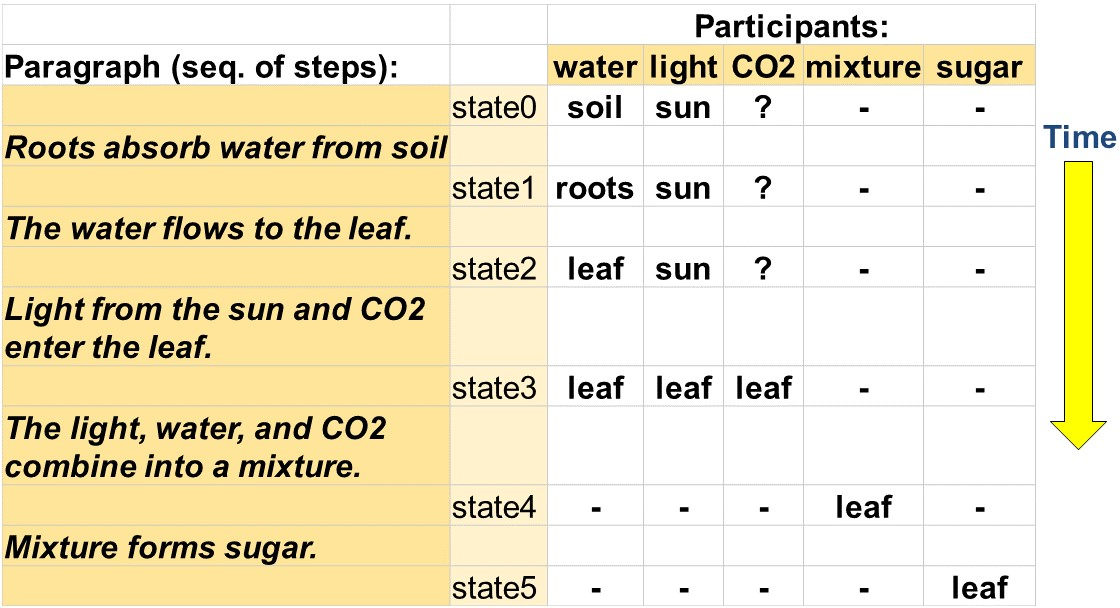
\includegraphics[width=8cm]{participant-grid-simple.JPG}
\caption{ProPara participant state change grid.}
\label{fig:participant-grid}
\end{figure}

To evaluate our system, we use the ProPara procedural text benchmark 
which contains 488 crowd-sourced paragraphs and 3100 sentences total. 
This data set is comprised of procedural text paragraphs covering different 
topics together with a human annotated table that describes the state 
(location and existence) of entities in this paragraph. Figure 
\ref{fig:participant-grid} shows an instance of the training data which 
constitutes of a paragraph about photosynthesis and the annotated state 
change grid. The state change grid contains information about where an 
entity (e.g. water or light) is at each step. Note that "?" indicates the 
location is unknown, and "-" indicates the entity doesn't exist during that step.

\section{Model and Implementation}

TODO

\section{Evaluation and Results}

During testing the system will 4 categories of questions from the output 
state change grid: 

\begin{enumerate}
  \item What are the Inputs? That is, which participants existed before the 
  	  procedure began
  \item What are the Outputs? That is, which participants existed after 
	  the procedure ended?
  \item What are the Conversions? That is, which participants were 
  	  converted to which other participants?
  \item What are the Moves? That is, which participants 
	   moved from one location to another?
\end{enumerate}

Note that these questions are templated, meaning they can be deterministically 
answered using the output state grid. The evaluation code was made available 
at \url{https://github.com/allenai/aristo-leaderboard/tree/master/propara} by 
the AI2 team. The code outputs precision, recall and F1 score for each 
question category.

\section{Conclusion}

TODO

\bibliography{emnlp2018}
\bibliographystyle{acl_natbib_nourl}

\end{document}
